\documentclass[10pt, a4paper]{article}
\usepackage[utf8]{inputenc}
\usepackage[spanish]{babel}

\usepackage{varwidth}
\usepackage{graphicx}
\usepackage{eurosym} % para el euro

\usepackage[T1]{fontenc} % Use 8-bit encoding that has 256 glyphs


\usepackage[hmarginratio=1:1,top=32mm,columnsep=20pt]{geometry} % Document margins
\usepackage[hang, small,labelfont=bf,up,textfont=it,up]{caption} % Custom captions under/above floats in tables or figures

\usepackage{float} % Required for tables and figures in the multi-column environment - they need to be placed in specific locations with the [H] (e.g. \begin{table}[H])

\usepackage{hyperref} % For hyperlinks in the PDF


\usepackage{amsmath,amssymb}


\usepackage{titlesec} % Allows customization of titles
\renewcommand\thesection{} % Roman numerals for the sections
\renewcommand\thesubsection{\alph{subsection}} % Roman numerals for subsections
\titleformat{\section}[block]{\large\scshape\centering}{\thesection}{1em}{} % Change the look of the section titles
\titleformat{\subsection}[block]{\large}{\thesubsection.}{1em}{} % Change the look of the section titles

\usepackage{fancyhdr} % Headers and footers
\pagestyle{fancy} % All pages have headers and footers
\fancyhead{} % Blank out the default header
\fancyfoot{} % Blank out the default footer
\fancyhead[C]{Sergio García Prado $\bullet$ Marzo 2016 $\bullet$ Modelos para la Toma de Decisiones $\bullet$ Tarea 1} % Custom header text
\fancyfoot[RO,LE]{\thepage} % Custom footer text

%----------------------------------------------------------------------------------------
%	TITLE SECTION
%----------------------------------------------------------------------------------------

\title{\vspace{-15mm}\fontsize{24pt}{10pt}\selectfont\textbf{Modelos para la Toma de Decisiones: Tarea 1}} % Article title

\author{
\large
\textsc{Sergio García Prado}\\[2mm] % Your name
\normalsize Universidad de Valladolid \\ % Your institution
\vspace{-5mm}
}
\date{}

%----------------------------------------------------------------------------------------

\begin{document}

	\maketitle % Insert title

	\thispagestyle{fancy} % All pages have headers and footers

%----------------------------------------------------------------------------------------
%	TEXT
%----------------------------------------------------------------------------------------

    \section{Ejercicio 1}

        \begin{figure}[H]
        \centering
            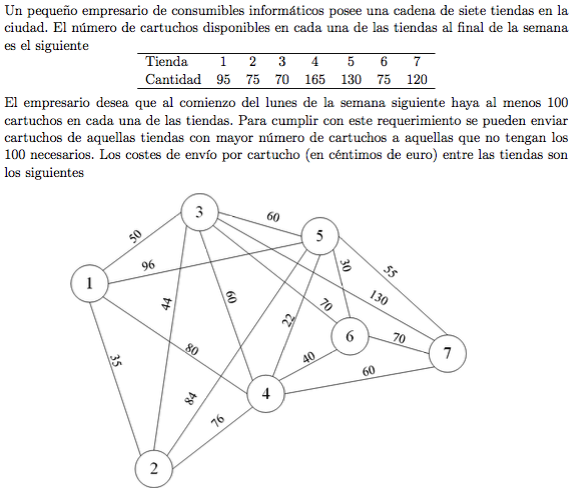
\includegraphics[width=0.75\textwidth]{res/Exercise_1.png}
        \end{figure}

		\subsection{Determinar la mejor manera de distribuir los cartuchos entre las tiendas.}

			\paragraph{}
			Lo primero que haremos será modelar el enunciado del problema. Se ha tenido en cuenta el detalle que indica que los envíos de cartuchos tan solo son posibles desde las tiendas que tienen un exceso de cartuchos (más de 100) a las que tienen déficit (menos de 100).

			\paragraph{}
			La notación que se va a utilizar para denotar las variables es la siguiente:
			\paragraph{}
			\(x_{ij}\) = Número de cartuchos enviados desde la tienda \(i\) hasta la tienda \(j\). \(\quad i=4,5,7. \quad j=1,2,3,6.\)

			\paragraph{}
			Notese que tal y como indica el enunciado del problema la función objetivo de este consistirá en minimizar la suma de costes necesarios para llegar al objetivo del número de cartuchos por tienda. Por tanto las restricciones asociadas al problema servirán para restringir el tanto el número de cartuchos que se pueden envíar a partir de una tienda de origen, como el número necesario de cartuchos que se necesitan en el caso de las tiendas de destino.

			\paragraph{}
			A continuación se muestra la modelización del problema:

			\[
			  \small
			  \begin{array}{r@{}r@{}r@{}r@{}r@{}r@{}r@{}r@{}r@{}r@{}l}
			    \text{Min} \quad z=	80x_{41} &{} + 76x_{42} &{} + 60x_{43} &{} + 40x_{46} &{} + 96x_{51} &{} + 84x_{52} &{} + 60x_{53} &{} + 30x_{56} &{} + 130x_{73} &{} + 70x_{76} &{} \\[\jot]
			    \text{sujeto a}\qquad 	x_{41} &{} +   x_{42} &{} +   x_{43} &{} +   x_{46} &{}   &{}   &{}   &{}   &{}   &{}   &{} \leq 65 \\
			                     	&{}  &{}  &{}  &{} x_{51} &{} + x_{52} &{} + x_{53} &{} + x_{56} &{}  &{}  &{} \leq 30 \\
								 	&{} &{}  &{}  &{}  &{} &{}  &{}  &{} x_{73} &{} + x_{76} &{} \leq 20 \\
								 	x_{41} &{} &{} &{} &{} + x_{51} &{} &{}  &{}  &{} &{}  &{} \geq 5 \\
								 	&{}  x_{42} &{}  &{} &{}  &{} + x_{52} &{}  &{}  &{} &{}  &{} \geq 25 \\
								 	 &{}  &{}  x_{43} &{}  &{}  &{}  &{} + x_{53} &{}  &{} + x_{73} &{}  &{} \geq 30 \\
								 	&{}  &{}  &{} x_{46} &{}  &{}  &{}  &{} + x_{56} &{}  &{} + x_{76} &{} \geq 25 \\
			     \multicolumn{10}{c}{x_{ij} \geq 0, \quad i=4,5,7. \quad j=1,2,3,6.}
			  \end{array}
			\]
			\paragraph{}
			La tabla simplex final resultante es la siguiente:

			\begin{figure}[H]
	        \centering
	            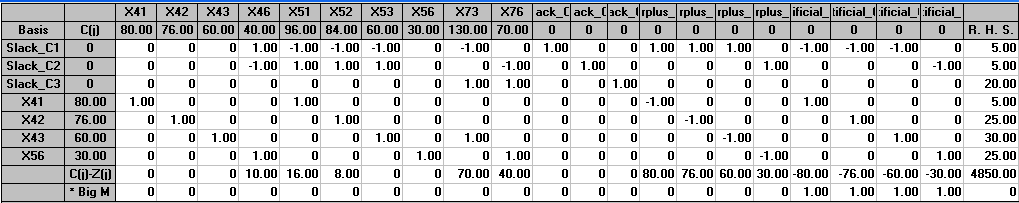
\includegraphics[width=\textwidth]{res/Exercise_1_pp_simplex_final.png}
	        \end{figure}

			\paragraph{}
			Si nos fijamos en la última columna objervamos que los valores que consiguen el óptimo de la función objetivo son:
			\(x_{41}^{*} = 5 \), \(x_{42}^{*} = 25 \), \(x_{43}^{*} = 30 \), \(x_{56}^{*} = 25 \) lo cual resulta en \(z^{*} = 4850 \).

			\paragraph{}
			\textbf{Solución:} La traducción de este resultado nos indica que para que el empresario pueda tener al menos 100 cartuchos en cada una de sus tiendas tendrá que envíar:

			\begin{itemize}
				\item 5 cartuchos de la tienda 4 a la tienda 1.
				\item 25 cartuchos de la tienda 4 a la tienda 2.
				\item 30 cartuchos de la tienda 4 a la tienda 3.
				\item 25 cartuchos de la tienda 5 a la tienda 6.
			\end{itemize}

			Esto le ocasionará un coste de 4850 céntimos de euro, es decir, 48.50\euro

		\subsection{?`En cuánto puede variar el coste de envío entre las tiendas 4 y 6 para que la solución Óptima calculada en el apartado (a) se mantenga? Razonar la respuesta.}

			\paragraph{}
			En este caso necesitamos conocer el intervalo de optimalidad asociado la modificación del valor de coste de la variable \(x_{46}\) en la función objetivo. Dado que esta variable es no básica (su valor es cero cuando el resultado de la función objetivo es óptimo) nos fijaremos en el valor \(z_{k}\) para la restricción inferior e infinito en la restricción superior. Por tanto el intervalo es \((30,\infty)\)

			\paragraph{}
			\textbf{Solución:} El coste de transportar cartuchos de la tienda 4 a la tienda 6 para que la solución encontrada siga siendo óptima puede reducirse en 10 centimos o aumentar indefinidamente. El motivo es que Enviarlos desde la tienda 5 tiene un coste de 30 centimos.


		\subsection{Sin realizar iteraciones, obtener la nueva solución si el número de cartuchos disponibles en la tienda número 3 disminuye a 65 y el de la tienda 5 aumenta a 135 unidades. Justificar la respuesta.}

			\paragraph{}
			Tenemos que realizar un análisis de sensibilidad debido a un cambio el vector del lado derecho (LD).


			\[
			b^{'0} = B^{-1}b^{'} =
			\begin{bmatrix}
			    5 \\
			    5 \\
				20 \\
				5 \\
				25 \\
				30 \\
				25
			\end{bmatrix}
			-5
			\begin{bmatrix}
			    1 \\
			    0 \\
				0 \\
				0 \\
				0 \\
				-1 \\
				0
			\end{bmatrix}
			+5
			\begin{bmatrix}
			    0 \\
			    1 \\
				0 \\
				0 \\
				0 \\
				0 \\
				0
			\end{bmatrix}
			=
			\begin{bmatrix}
			    0 \\
			    10 \\
				20 \\
				5 \\
				25 \\
				35 \\
				25
			\end{bmatrix}
			\]

			\paragraph{}
			Dado que todas las variables de este quedan positivas sabemos que la base anterior sigue siendo una solución básica factible, por tanto la nueva solución es:

			\(x_{41}^{*} = 5 \), \(x_{42}^{*} = 25 \), \(x_{43}^{*} = 35 \), \(x_{56}^{*} = 25 \) lo cual resulta en \[
				z^{'*} = z^{0} -5 *(-60) + 5*0 = 4850 + 300 = 5160
			\]

		\subsection{Sin resolver desde el principio el problema y utilizando la tabla simplex Óptima, determinar la nueva solución si el número de cartuchos de la tienda número 2 disminuye a 65 y el de la tienda 5 aumenta a 135 unidades. Justificar la respuesta.}

			\paragraph{}
			Tenemos que realizar un análisis de sensibilidad debido a un cambio el vector del lado derecho (LD).

			\[
			b^{'0} = B^{-1}b^{'} =
			\begin{bmatrix}
				5 \\
				5 \\
				20 \\
				5 \\
				25 \\
				30 \\
				25
			\end{bmatrix}
			-10
			\begin{bmatrix}
				1 \\
				0 \\
				0 \\
				0 \\
				-1 \\
				0 \\
				0
			\end{bmatrix}
			+5
			\begin{bmatrix}
				0 \\
				1 \\
				0 \\
				0 \\
				0 \\
				0 \\
				0
			\end{bmatrix}
			=
			\begin{bmatrix}
				-5 \\
				10 \\
				20 \\
				5 \\
				15 \\
				30 \\
				25
			\end{bmatrix}
			\]

			\paragraph{}
			En este caso el vector del lado derecho ha sido modificado dando lugar a que algunas de sus componentes pasen a ser negativas, por lo que ya no será una solución básica factible por lo que tendremos que realizar iteracciónes hasta llegar otra vez a ella.

			\[
				z^{'*} = z^{0} -10 *(-76) +5*0 = 4850 + 760 = 5610
			\]

			El resultado de realizar iteracciones (sale la variable de holgura asociada a la primera restricción y entra \(x_{53}\) da como resultado óptimo:
			\(x_{41}^{*} = 5 \), \(x_{42}^{*} = 35 \), \(x_{43}^{*} = 25 \), \(x_{56}^{*} = 25 \), \(x_{53}^{*} = 5 \) lo cual resulta en \[
				z^{*} = 5610
			\]

		\subsection{Escribir el problema dual del formulado en el apartado (a)}

			\paragraph{}
			El problema dual asociado al formulado en el apartado (a) es el siguiente. Consiste en hacer que las restricciones pasen a ser variables y viceversa, aplicando los correspondientes cambios.


			\[
			  \begin{array}{r@{}r@{}r@{}r@{}r@{}r@{}r@{}l}
			    \text{Max} \quad z = 65w_{1} &{} +30w_{2} &{} + 20w_{3} &{} + 5w_{4} &{} + 25w_{5} &{} + 30w_{6} &{} + 25w_{7} &{} \\[\jot]
			    \text{sujeto a}\qquad 	w_{1} &{} 		&{} 		&{} + w_{4} &{} &{} &{}  &{} \leq 80 \\
			                     		w_{1} &{} 		&{} 		&{} 		&{} + w_{5}&{} &{}  &{} \leq 76 \\
								 		w_{1} &{} 		&{} 		&{} 		&{} &{} + w_{6}&{}  &{} \leq 60 \\
								 		w_{1} &{} 		&{} 		&{} 		&{} &{} &{} + w_{7} &{} \leq 40  \\
								 		      &{} w_{2} &{} 		&{} + w_{4}	&{} &{} &{}  &{} \leq 96 \\
											  &{} w_{2} &{} 		&{} 		&{} + w_{5} &{} &{}  &{} \leq 84 \\
											  &{} w_{2} &{} 		&{} 		&{} &{} + w_{6}&{}  &{} \leq 60 \\
											  &{} w_{2} &{} 		&{} 		&{} &{} &{} + w_{7} &{} \leq 30 \\
											  &{} 		&{} w_{3} 	&{} 		&{} &{} + w_{6} &{}  &{} \leq 130 \\
											  &{} 		&{} w_{3} 	&{} 		&{} &{} &{} +w_{7} &{} \leq 70 \\
			     \multicolumn{6}{c}{w_{1}, w_{2}, w_{3} \leq 0, w_{4}, w_{5}, w_{6}, w_{7} \geq 0}


			  \end{array}
			\]

		\subsection{Resolver el problema del apartado (e) utilizando las condiciones de holgura complementaria. ?`Es única la solución? Razonar la respuesta.}

			\paragraph{}
			Aplicando el teorema de holgura complementaria llegamos a las siguientes ecuaciones(se han omitido aquellas que iban a ser triviales al dar valores a las variables \(x_{ij}\)):

			\[
			\begin{split}
				(w_{1} + w_{4} - 80)x_{41} = 0 \\
				(w_{1} + w_{5} - 76)x_{41} = 0 \\
				(w_{1} + w_{6} - 60)x_{41} = 0 \\
				(w_{2} + w_{7} - 30)x_{41} = 0 \\
			\end{split}
			\]

			\paragraph{}
			Ahora sustituimos \(x_{ij}\) por los valores óptimos del problema primal:

			\[
			\begin{split}
				(w_{1} + w_{4} - 80)5 = 0 \\
				(w_{1} + w_{5} - 76)25 = 0 \\
				(w_{1} + w_{6} - 60)30 = 0 \\
				(w_{2} + w_{7} - 30)25 = 0 \\
			\end{split}
			\]
			\paragraph{}
			Operando llegamos al siguiente resultado, que como vemos es un sistema compatible indeterminado, por tanto tiene infinitas soluciones:

			\[
			\begin{split}
				w_{1} + w_{4} = 80 \\
				w_{1} + w_{5} = 76 \\
				w_{1} + w_{6} = 60 \\
				w_{2} + w_{7} = 30 \\
			\end{split}
			\]

			\paragraph{}
			Una solucion, por tanto, es: \(w_{4}^{*} = 80 \), \(w_{5}^{*} = 76 \), \(w_{6}^{*} = 60 \), \(w_{7}^{*} = 30 \)lo cual resulta en \(z^{*} = 4850\)

		\subsection{Suponer ahora que los cartuchos se pueden enviar entre todas las tiendas conectadas. Modelizar, sin resolver, este nuevo problema.}

			\paragraph{}
			Ahora que permitiremos que se envíen cartuchos desde cualquier tienda a cualquier otra necesitamos tener dos variables para cada uno de los dos sentidos que puede tomar una arista. No hay problema de que se envían y reciban simultaneamente por la misma arista ya que la función objetivo penaliza esta situación.

			\paragraph{}
			Al igual que en el caso anterior la notación que se va a utilizar para denotar las variables es la siguiente:

			\paragraph{}
			\(x_{ij}\) = Número de cartuchos enviados desde la tienda \(i\) hasta la tienda \(j\). \(\quad i=(1,7) \quad j=(1,7).\)

			\[
			    \small
			    \begin{split}
				    \text{Min} \quad z = 35(x_{12}+x_{21}) + 50(x_{13}+x_{31}) + 80(x_{14}+x_{41}) + 96(x_{15}+x_{51}) \\
			        + 44(x_{23}+x_{32}) + 76(x_{24}+x_{42})+ 84(x_{25}+x_{52}) + 60(x_{34}+x_{43}) \\
			        + 60(x_{35}+x_{53}) + 70(x_{36}+x_{63}) + 130(x_{37}+x_{73}) + 22(x_{45}+x_{54})  \\
			        + 40(x_{46}+x_{64}) + 60(x_{47}+x_{74}) + 30(x_{56}+x_{65}) + 55(x_{57}+x_{75}) \\
			        + 70(x_{67}+x_{76})  \\
			                            \\
			        \text{sujeto a}
			        \qquad 	x_{21} - x_{12} + x_{31} - x_{13} + x_{41} - x_{14} + x_{51} - x_{15}  \geq 5  \\
			        \qquad 	x_{12} - x_{21} + x_{32} - x_{23} + x_{42} - x_{24} + x_{52} - x_{25}  \geq 25  \\
			        \qquad 	x_{13} - x_{31} + x_{23} - x_{32} + x_{43} - x_{34} + x_{53} - x_{35} + x_{63} - x_{36} + x_{73} - x_{37} \geq 30  \\
			        \qquad 	x_{14} - x_{41} + x_{24} - x_{42} + x_{34} - x_{43} + x_{54} - x_{45} + x_{64} - x_{46} + x_{74} - x_{47} \geq -65  \\
			        \qquad 	x_{15} - x_{51} + x_{25} - x_{52} + x_{35} - x_{53} + x_{45} - x_{54} + x_{65} - x_{56} + x_{75} - x_{57}  \geq -30  \\
			        \qquad 	x_{36} - x_{63} + x_{46} - x_{64} + x_{56} - x_{65} + x_{76} - x_{67}  \geq 25  \\
			        \qquad 	x_{37} - x_{73} + x_{47} - x_{74} + x_{57} - x_{76} + x_{67} - x_{76}  \geq -20  \\
			        \qquad  x_{ij} \geq 0, i=1,2,3,4,5,7. \quad j=1,2,3,4,5,6,7.
			    \end{split}
			    \]

    \section{Ejercicio 2}

        \begin{figure}[H]
        \centering
            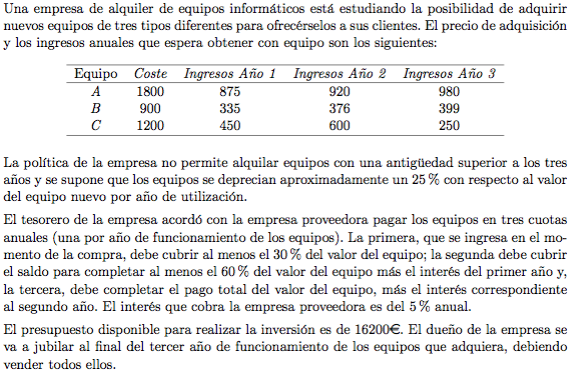
\includegraphics[width=0.75\textwidth]{res/Exercise_2.png}
        \end{figure}

		\subsection{Formular un modelo de PL para determinar el plan Óptimo de compras y de pagos que maximice los beneficios al final del periodo de tres años.}

			\paragraph{}
			El problema se ha formulado entendiendo del enunciado los siguiente: Se puede comprar equipos tan solo al principio de la planificación. Estos se pagarán en tres plazos, el primero en el momento de la compra de al menos el 30\%, el segundo del al menos el 60\% cuando haya pasado un año y el ultimo cuando haya pasado otro año completando el importe restante. Además cada año se paga un 5\% de interés por el porcentaje de pago que todavía no se ha completado. Los equipos se pueden vender en cualquier momento devaluandose un 25\% cada año. El presupuesto disponible al principio de la planificación es de 16200 \euro y cada año se pueden utilizar los ingresos para pagar los equipos.

			\paragraph{}
			Para modelizar el problema según el razonamiento expuesto se han utilizado las siguientes variables:

			\begin{itemize}
				\item \(A = \) Número de equipos comprados al principio de la planificación del tipo A

				\item \(B = \) Número de equipos comprados al principio de la planificación del tipo B.

				\item \(C = \) Número de equipos comprados al principio de la planificación del tipo C.

				\item \(p_{i} = \) Cantidad de euros que se pagará al inicio del año i por los equipos intereses. \(i = (1,2,3)\)
			\end{itemize}

			\paragraph{}
			La modelización del problema es por tanto la siguiente:

			\[
			  \begin{array}{r@{}r@{}r@{}r@{}r@{}r@{}r@{}l}
			    \text{Max} \quad z = 	5025A	&{} + 2235B		&{} + 2800C 	&{}	-P1 	&{} -P2		&{} -P3 	&{}\\[\jot]
			    \text{sujeto a}\qquad 	1800A 	&{} + 900B		&{} + 1200C	&{} 		&{}			&{}			&{}	\leq 16200 \\
			                     		540A 	&{} + 270B		&{} + 360C	&{}	-P1		&{}			&{}			&{}	\leq 0 \\
								 		1134A 	&{} + 567B		&{} + 756C	&{}	-0.63P1	&{}	-P2		&{} 		&{}	\leq 0 \\
								 		1984.5A &{} + 992.25B	&{} + 1323C	&{}-1.1025P1&{}	-1.05P2	&{}  -P3	&{}	= 0  \\
			     \multicolumn{6}{c}{ A, B, C, P1, P2, P3 \geq 0}


			  \end{array}
			\]

			\paragraph{}
			Tanto los coeficientes de coste con la matriz de restricciones se han operado para simplificar el resultado. Las expresiones sin simplificar son las siguientes:
			\[
				\begin{split}
					\text{Max} z = (875 + 920 + 980 + 1800 * 0.25 + 1800)A \\
					+ (335 + 376 + 399 + 900 * 0.25 + 900)B \\
					+(450 + 600 + 250 + 1200 * 0.25 + 1200)C \\
					-(P1 + P2 + P3) \\ \\
					1800A + 900B + 1200C <= 16200 \\
					0.3(1800A + 900B + 1200C) <= P1 \\
					0.6*1.05((1800A + 900B + 1200C)-P1) <= P2 \\
					1.05(1.05((1800A + 900B + 1200C)-P1)-P2) = P3\\
				\end{split}
			\]

			\paragraph{}
			La tabla simplex final resultante es la siguiente:

			\begin{figure}[H]
			\centering
				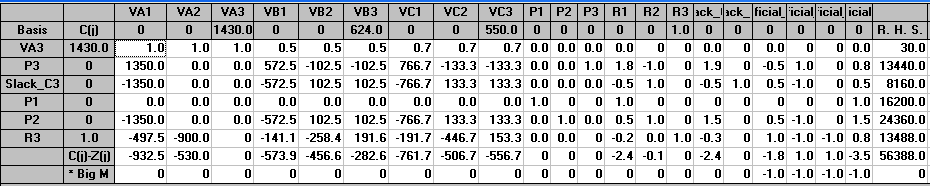
\includegraphics[width=\textwidth]{res/Exercise_2_pp_simplex_final.png}
			\end{figure}

		\subsection{?`Cuál es el plan Óptimo?}

			\paragraph{}
			\textbf{Solución:} El plan óptimo es la compra de \textbf{9 equipos de tipo A}, los cuales se pagarán en su totalidad en el primer plazo, consiguiendo así una reducción de costes debido a que no habrá que pagar intereses por la compra. Con esto se obtiene un beneficio de \textbf{29025\euro}.

		\subsection{Escribir el problema dual del formulado en el apartado (a).}

			\paragraph{}
			El problema dual asociado al formulado en el apartado (a) es el siguiente. Consiste en hacer que las restricciones pasen a ser variables y viceversa, aplicando los correspondientes cambios.

			\[
			  \begin{array}{r@{}r@{}r@{}r@{}l}
			    \text{Min} \quad z = 16200w_{1} \\[\jot]
			    \text{sujeto a}\qquad 	1800w_{1} 	&{}+540w_{2}&{}	+1134w_{3} 		&{} +1984.5w_{4} 	\geq 5025 \\
			                     		900w_{1} 	&{}+270w_{2}&{}	+567w_{3} 		&{} +992.25w_{4}	\geq 2 \\
								 		1200w_{1} 	&{}+360w_{2}&{} +756w_{3}		&{} +1323w_{4}		\geq 2 \\
								 		  			&{}º   w_{2}&{} +0.63w_{3}		&{} +1.1025w_{4}	\leq 1  \\
								 		  			&{} 		&{} 	w_{3}		&{} +1.05w_{4}		\leq 1 \\
										    		&{} 		&{} 				&{} w_{4} 			\leq 1 \\
			     \multicolumn{3}{c}{ w_{2},w_{2},w_{3} \geq 0,  w_{4} s.r.s}
			  \end{array}
			\]


		\subsection{Determinar la solución Óptima del problema formulado en (c) utilizando las condiciones de holgura complementaria.}

			\paragraph{}
			Aplicando el teorema de holgura complementaria llegamos a las siguientes ecuaciones(se han omitido aquellas que iban a ser triviales al dar valores a las variables):
			\[
			\begin{split}
				(1800w_{1} + 540w_{2} + 1134w_{3} + 1984.5w_{4} - 5025)A = 0 \\
				(w_{2} +0.63w{3} + 1.1025w_{4} - 1)p_{1} = 0 \\
			\end{split}
			\]

			Sustituyendo el las variables del problema primal por sus resultados óptimos llegamos a un sistema compatible indeterminado que por tanto tiene infinitas soluciones, una de ellas es: \(w_{1}^{*} = 1.79 \), \(w_{4}^{*} = 0.91 \), lo cual resulta en \(z^{*} = 29025\)


		\subsection{Interpretar la variable dual asociada a la restricción del presupuesto disponible.}

			\paragraph{}
			Esta variable indica la variación producida por un incremento unitario en el presupuesto inicial, es decir, por cada euro más de inversión obtendremos un beneficio de 1.79 \euro más al final de los tres años.


\end{document}
